\documentclass{article}
\usepackage[utf8]{inputenc}
\usepackage{apacite}
\usepackage{graphicx}
\graphicspath{ {./image/} }
\topmargin 0.0cm
\oddsidemargin 0.0cm
\textwidth 16cm 
\textheight 21cm
\footskip 1.0cm

\title{Extant prehistoric rituals in Central and Southeastern Europe}
\author{Miron Stratan}
%%\date{February 2019}

\begin{document}

\maketitle

\bibliographystyle{apacite}

\section{The meaning of boiled grains: the hidden story of polenta}

This author contends that recipes for staple foods could in fact be very old. 
One could argue that polenta can't be an example of an ancient food in Europe, since is made out of maize. In turn, the maize plant was domesticated in the Americas (reference pending) and was brought to Europe at around 1600 AD (reference pending) where slowly grew in popularity as a crop, due to superior productivity and because can be used as fodder.
Even if polenta contains only three ingredients (coarse maize flour, salt and water), one needs to pay attention to the process to avoid uncooked lumps or a burned bottom. Anyone who tried to cook polenta knows it requires a lot of stirring, from the start to avoid the forming of lumps and to continue stirring from time to time to allow for an even boiling. But is when one experiments with maize flour of different particle size, one could realize, that despite the effort put in stirring, the best quality polenta is obtained from a flour with a specific particle size: if the flour is too coarse it wouldn't stick together, if ground into fine powder, maize would require more water to evenly boil, and the result is too liquid.
This is when one could start to suspect that the recipe was perfected for other type of corn and maize is a replacement option.
Before inferring what is maize replaceing in this recipe, a detour in linguistics is proposed.
In Southeastern Europe this dish is  known under a name of uncertain ethimology: mamalingë (Albanian), мамалига (Bulgarian), mămălígă (Romanian), μαμαλίνγα (Greek), mamaliga (Hungarian), mamaljuga (Serbo-Croatian), mamalyg (Rusyn), 

\section{The game of astragals}


In the search for extant prehistoric rituals in Central and Southeastern Europe, stopping by what apparently is a child activiy might seem odd, but let's examine this game being played until recently throughout the region \cite{Capidan1934}. 
A first approach could be linguistic, as the game is known under variants of the same name in Albanian, Bulgarian, Romanian and Serbian \cite{DER1966}:  asik, ar{\c{s}}ic, or arsik, words etymologically linked to the Turkish word a{\c{s}}ik, so it could potentially be regarded as a legacy of the Ottoman Empire. \textit{An open question is how many similarities the local astragals game had with the Turkish or Tartar games called a{\c{s}}ik.}

Looking at the game itself, with kids taking turns at juggling and interpreting the occurring formations of fallen knuckle-bones, then our line of thinking glides from the profane plane, or ludic in this case, to the mystical world, as astragals are also strongly tied in the Mediterranean antiquity to divination rituals \cite{mazzorin2013ancient}, \cite{holmgren2002money}.

Turning to archaeology, one can see astragal finds from the tip of the Balkan peninsula \cite{Trantalidou2019} to the Carpathian basin \cite{Filip&Mladen2017} and from the Lower Danube \cite{Kogalniceanu2015} up to the North Pontic forest-steppe \cite{Gry2013}. As early as the fifth millennium BC people seem to become fascinated with the diminutive back feet bones of domesticated ruminants, sheep, goats and later of cattle \cite{bailey2002balkan}. The finds are related to burials and household contexts \cite{Leshtakov2018} and various uses were inferred in the above mentioned papers: as ornaments, with holes for pendants, bead strings or belts, entire or faceted, and also grouped in sets potentially used in rituals.

People were clearly attaching specific meanings to the shape of astragals and were creating replicas of these bones from other materials: clay, stone (Trantalidou, 2019, p. 62)  or even high-value materials, like the gold astragal found in the Copper Age burial from Varna (Bailey 2000, p. 184).

Cognitive Archaeology could be applied to gain an understanding of the meaning of the astragal finds from the Copper Age and the Bronze Age, but more insights in the associated rituals come from the Iron Age writing and art. We learn of the Greek use of astragals: a popular game, as seen on this classical Lekythos vase \cite{WaltersMuseum},

\begin{center}
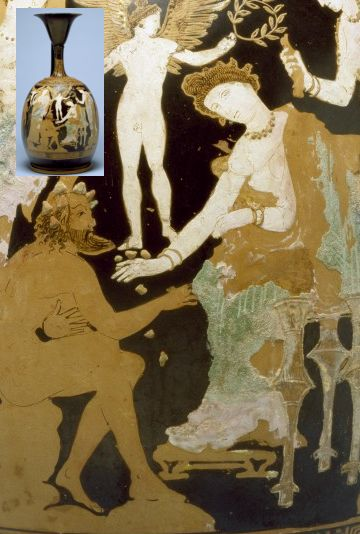
\includegraphics[scale=0.5]{Lekythos}

Lekythos with Knucklebone Players and Attendants, The Walters Art Museum collection, Creative Commons CC0 1.0
\end{center}

And there is \textbf{astragalomanteia}, a divination ritual, in which astragals were cast and the associated numbers were used to select a corresponding oracular inscription (Trantalidou 2019, p. 64; Mazzorin \& Minniti, 2013, p. 372).

The emerging pattern, that one can see from Late Neolithic until modern times, is an association of pastoral activities with the use of astragals in ludic and divination rituals. Several burials have children being interred with sets of astragals (Bailey 2000, p. 264; Gryshchuk 2013, p. 24) as if these bones were part of the passage ritual, as Trantalidou suggests also for the astragal votive offerings at the nymph shrine a cave on Mount Helicon in Boeotia (Trantalidou 2019, loc. cit.).


\bibliography{ref}
\end{document}
